\documentclass[a4paper,12pt]{article}
\usepackage[style=authoryear,sorting=ynt, maxbibnames=2]{biblatex}
\usepackage[unicode, draft=false]{hyperref}
\usepackage[scale=0.9]{geometry}
\usepackage{xcolor}
\usepackage{graphicx}
\usepackage{amsmath}
\usepackage{lmodern}

\title{Teleprocessamento e Redes - Relatório do trabalho final}
\author{
  Leonardo Ribeiro Santiago (120036072) \\
  João Matheus Nascimento Gonçalves (120023786) \\
  Esteves Emmanuel Melo Ferreira (117209640) }

\newcommand{\code}[1]{\texttt{#1}}

\date{}

\begin{document}

\maketitle

\section{Introdução}

Neste relatório iremos responder as perguntas relacionadas ao trabalho final. O código está disponível no seguinte repositório do github: {\color{blue} \href{https://github.com/o-santi/redes}{github.com/o-santi/redes}}.

Para reproduzir os resultados, deve-se instanciar uma máquina virtual Ubuntu usando Vagrant, assim como descrito em {\color{blue} \href{https://github.com/kaichengyan/mininet-vagrant}{github.com/kaichengyan/mininet-vagrant}}. Uma vez dentro da VM, clonamos o repositório git para uma pasta interna, e rodamos o arquivo \code{run.sh}.
\begin{verbatim}
  git clone -b entrega-preliminar https://github.com/o-santi/redes.git ~/redes
  cd ~/redes/bufferbloat
  chmod +x ./run.sh
  sudo ./run.sh
\end{verbatim}

Isto irá rodar os dois casos de teste (\code{max\_queue=20} e \code{max\_queue=100}) e gerar os gráficos citados neste relatório.

\section{Parte 2}

\subsection{Qual é o tempo médio de busca da página da web e seu desvio padrão quando q=20 e q=100?}

No caso \code{q=20}, o tempo médio de busca da página é de 3,30 segundos, com um desvio padrão de 0,82.
\begin{figure}[h!]
  \centering
  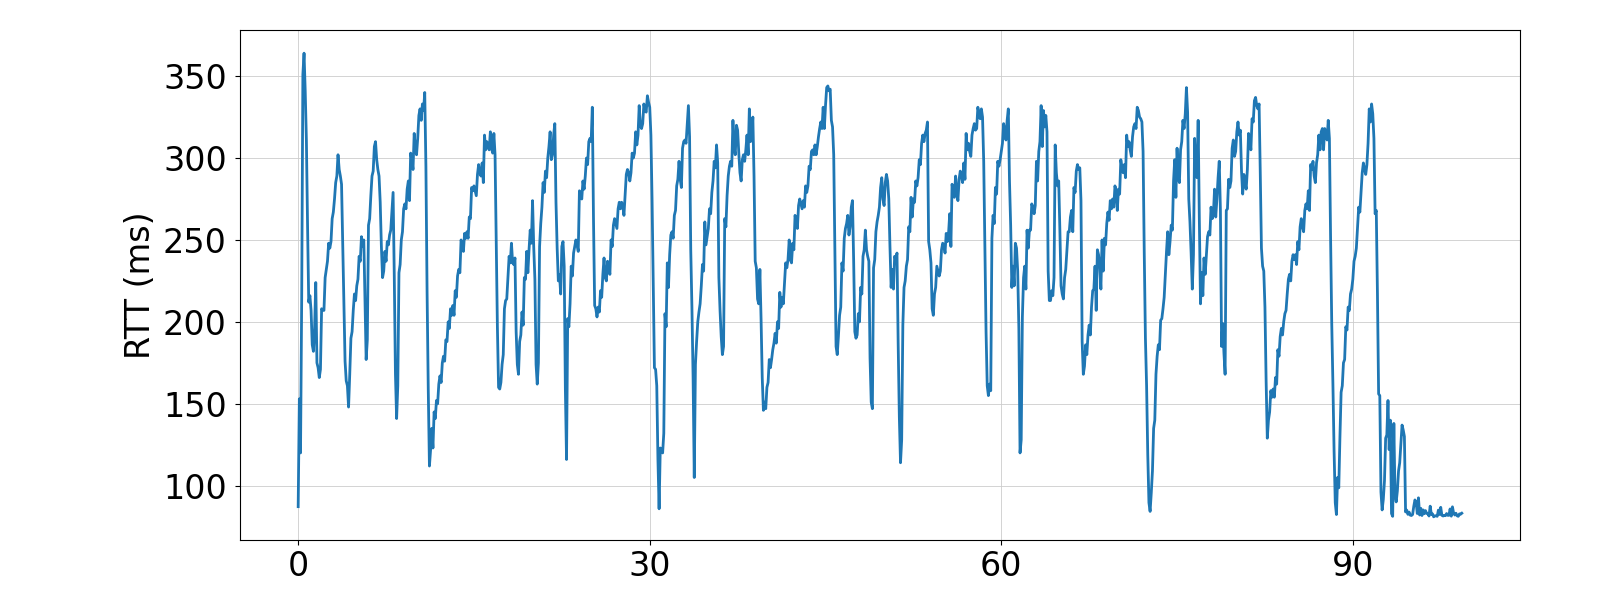
\includegraphics[width=0.5\columnwidth]{./bufferbloat/bb-q20/reno-rtt-q20.png}
  \caption{Tempo de resposta dos pings ao longo da duração do teste.}
  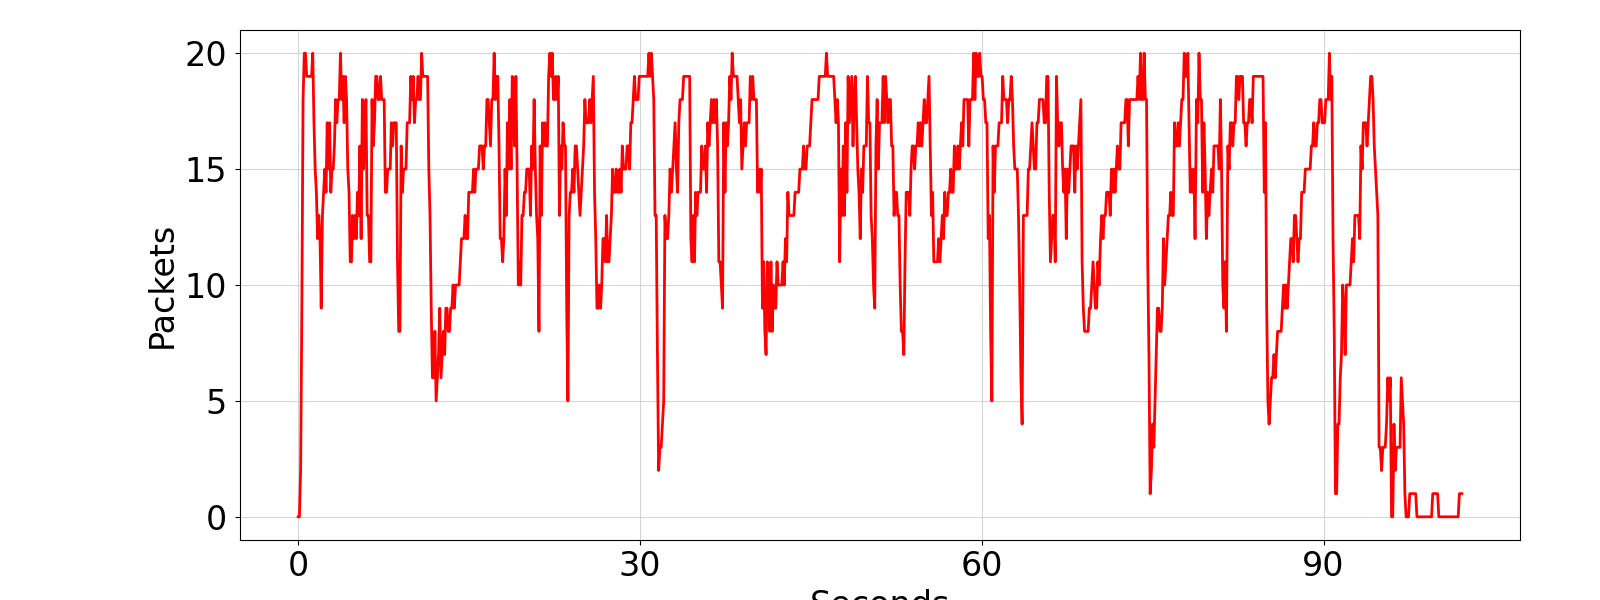
\includegraphics[width=0.5\columnwidth]{./bufferbloat/bb-q20/reno-buffer-q20.png}
  \caption{Número de pacotes na fila do switch ao longo do teste.}
\end{figure}

\newpage

Já no caso \code{q=100}, o tempo médio é de 9,96 segundos, com um desvio padrão de 3,17.

\begin{figure}[h!]
  \centering
  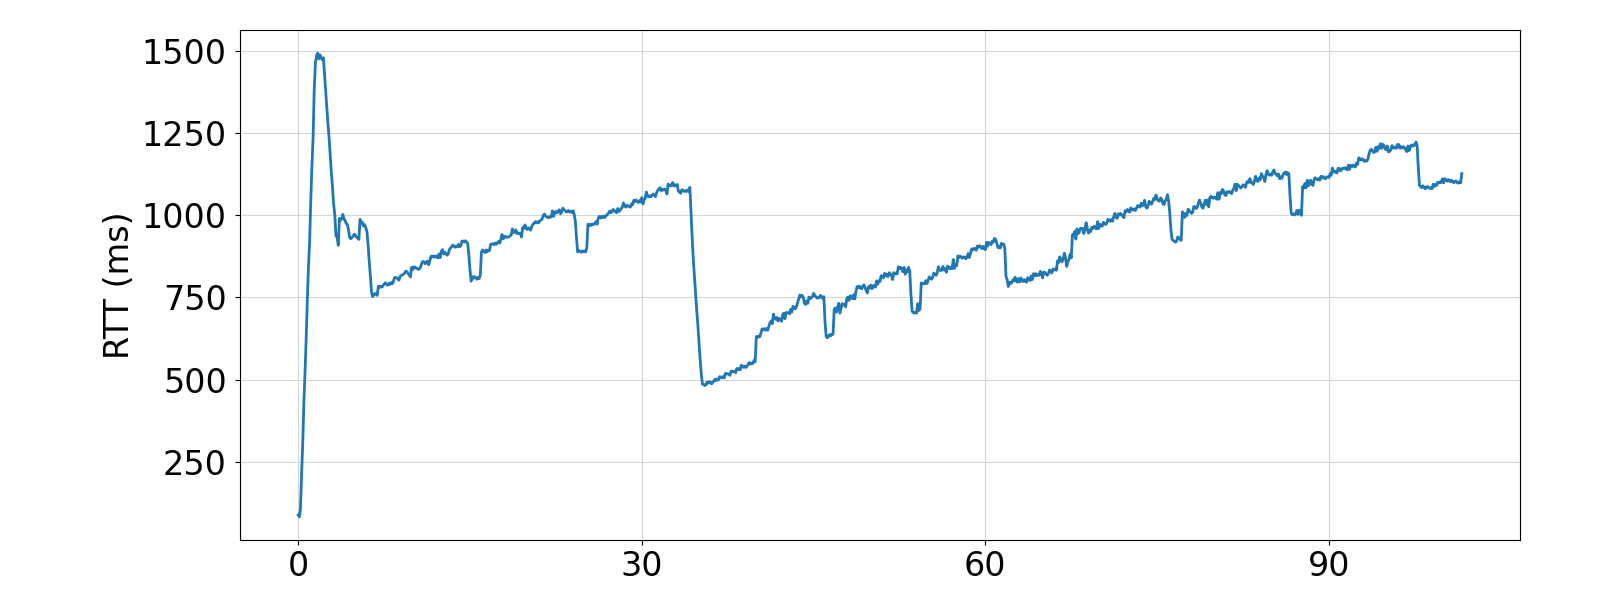
\includegraphics[width=0.5\columnwidth]{./bufferbloat/bb-q100/reno-rtt-q100.png}
  \caption{Tempo de resposta dos pings ao longo da duração do teste.}
  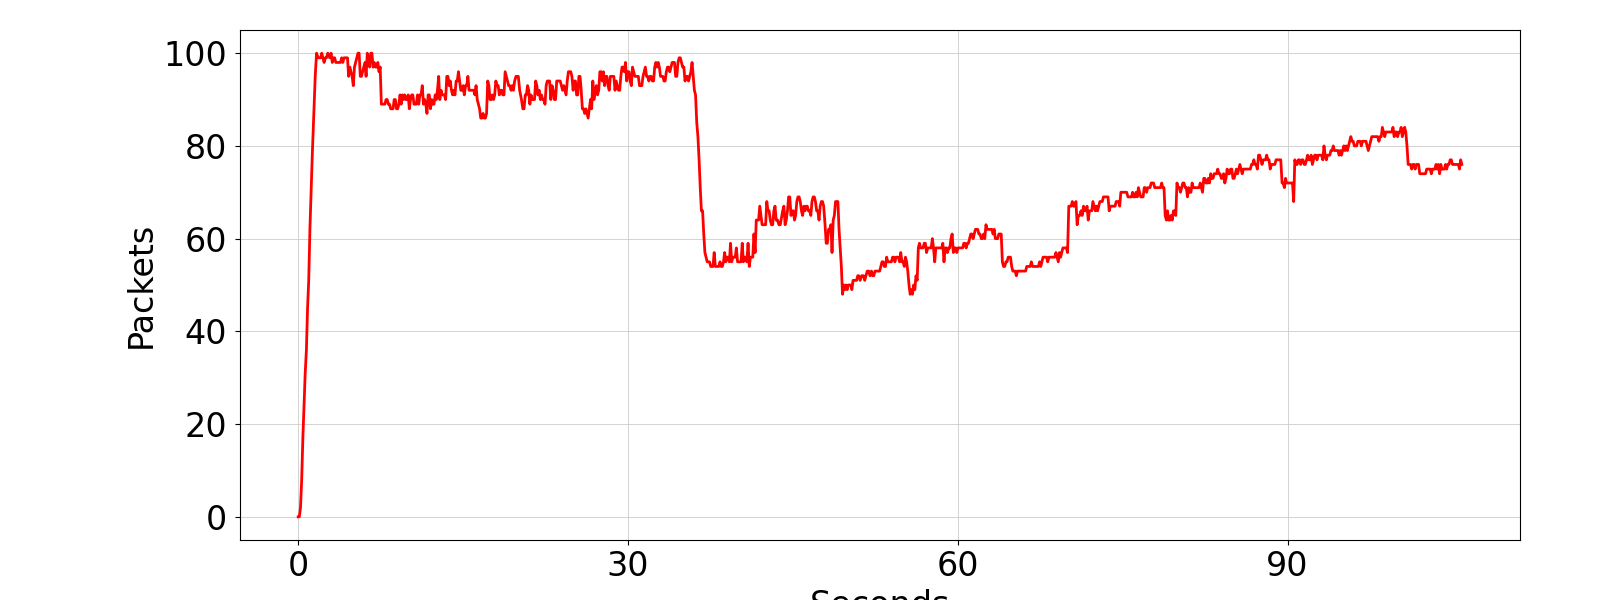
\includegraphics[width=0.5\columnwidth]{./bufferbloat/bb-q100/reno-buffer-q100.png}
  \caption{Número de pacotes na fila do switch ao longo do teste.}
\end{figure}

\subsection{Por que você vê uma diferença nos tempos de busca de páginas da Web com buffers de roteador curtos e grandes?}

A diferença pode ser explicada pela maior quantidade de pacotes que entram na fila, fazendo com que a janela de congestão da conexão TCP aumente, fazendo com que os pacotes passem mais tempo na fila esperando para serem transmitidos.

Ao diminuir o tamanho da fila para 20, os pacotes param de acumular como antes, fazendo com que o tempo que um pacote deve esperar na fila seja reduzido.

\subsection{Bufferbloat pode ocorrer em outros lugares, como sua placa de interface de rede (NIC). Verifique a saída de ifconfig eth0 de sua VM mininet. Qual é o comprimento (máximo) da fila de transmissão na interface de rede relatada pelo ifconfig? Para esse tamanho de fila, se você assumir que a fila é “drenada” a 100 Mb/s, qual é o tempo máximo que um pacote pode esperar na fila antes de sair da NIC?
}

Rodando \code{h1 ifconfig} de dentro da mininet, vemos que o parâmetro \code{txqueuelen} da interface principal \code{h1-eth0} é de 1000 pacotes, com \code{mtu=1500 bytes}.

Isso significa que, se um pacote entrar na última posição da fila, ele deve esperar todos os 999 pacotes transmitirem, e depois esperar o tempo da sua própria transmissão. O tempo máximo de transmissão de um pacote, na velocidade de \code{100Mb/s} é de $\frac{1000 * 1500 * 8}{100.000.000} \text{ segundos} = \frac{15 * 8}{1000} \text{ segundos} \approx 0,12 \text{ segundos} $. 

\subsection{Como o RTT relatado pelo ping varia com o tamanho da fila? Descreva a relação entre os dois.}

Tanto no caso \code{q=20} quanto quando \code{q=100}, o \code{RTT} aumenta linearmente com o número de pacotes na fila. Isso se dá pois o tempo de transmissão na rede é constante, dado que o único gargalo é o switch principal. Assim, quanto mais pacotes na fila do switch, maior será o tempo que ele levará para ser transmitido, e portanto maior será o RTT.

\subsection{Identifique e descreva duas maneiras de mitigar o problema de bufferbloat.}

De modo geral, técnicas para mitigar o \textit{bufferbloat} podem ser separadas em duas categorias: as que visam melhorar a rede e as que visam melhorar as pontas da conexão.

Dos que visam melhorar a rede, vale ressaltar os algorítmos \code{CoDel} (\textit{Controled Delay}) e sua melhoria \code{FQ-Codel} (\textit{Fair/Flow Queue CoDel}), que está dentro da categoria de algoritmos de \textit{Active Queue Management} (\code{AQM}). Esse algoritmo busca controlar o limite do delay que os pacotes experienciam nas filas dos roteadores para um máximo de 5 millisegundos. Caso o número de pacotes aumente rapidamente, de forma que o delay passe desse \textit{threshold}, pacotes são descartados da fila até que o delay esteja dentro do limite aceitável.

Dos que visam melhorar as pontas da conexão, destaca-se uma implementação do protocolo TCP utilizando um algoritmo de congestão diferente do \code{Reno}: o \textit{Bottleneck Bandwidth and Round-trip propagation time} (\code{BBR}). Diferentemente do \code{Reno}, que utiliza a perda de pacotes para detectar congestionamento e baixas taixas de transmissão, o \code{BBR} constroi um modelo da rede, utilizandos amostras de pacotes para medir a taxa de transmissão e o \textit{Round Trip Time} (\code{RTT}).

\section{Parte 3}

Para gerar os dados utilizando o método BBR, usamos o script \code{bufferbloat/run\_bbr.sh}.

\subsection{Qual é o tempo médio de busca da página da web e seu desvio padrão quando q=20 e q=100?}
No caso \code{q=20}, o tempo médio de busca da página é de 2,47 segundos, com um desvio padrão de 1,27.

\begin{figure}[h!]
  \centering
  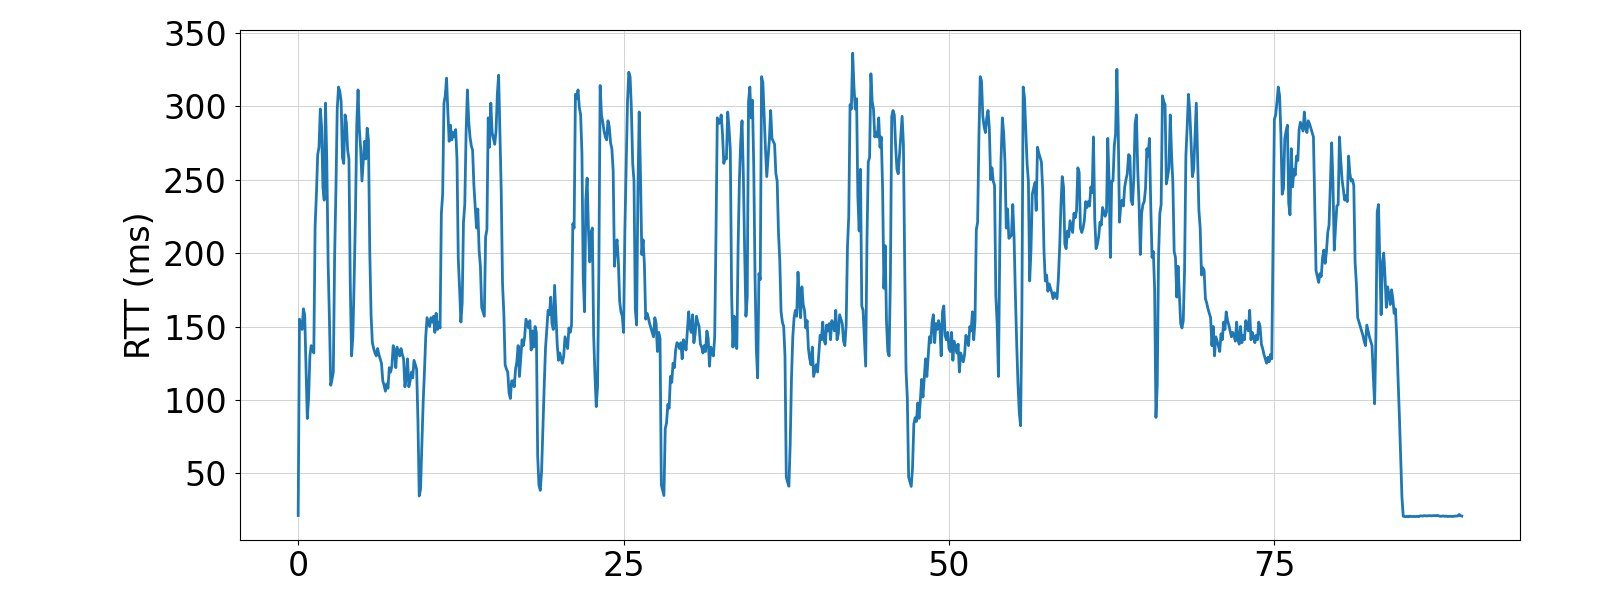
\includegraphics[width=0.7\columnwidth]{./bufferbloat/bb-q20/bbr-rtt.jpg}
  \caption{Tempo de resposta dos pings ao longo da duração do teste.}
  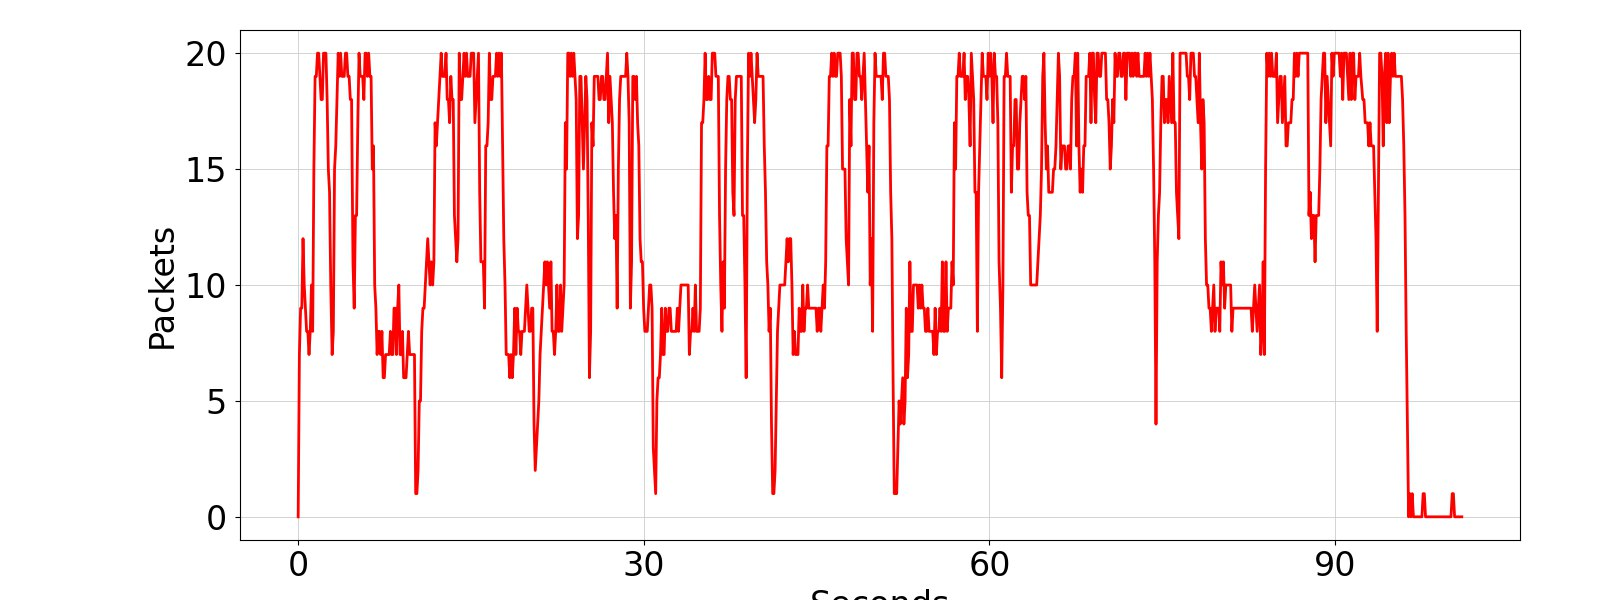
\includegraphics[width=0.7\columnwidth]{./bufferbloat/bb-q20/bbr-buffer.jpg}
  \caption{Número de pacotes na fila do switch ao longo do teste.}
\end{figure}

\newpage

No caso \code{q=100}, o tempo médio de busca da página é de 1,78 segundos, com um desvio padrão de 0,05.

\begin{figure}[h!]
  \centering
  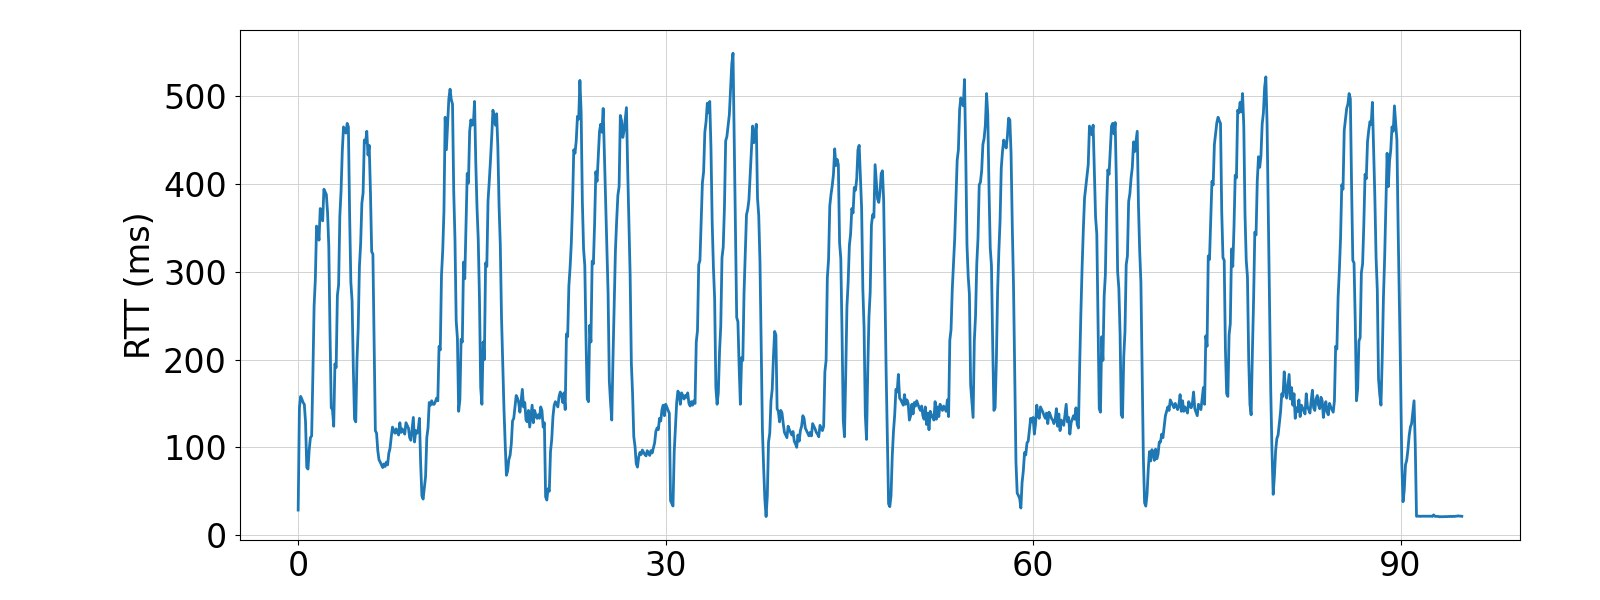
\includegraphics[width=0.7\columnwidth]{./bufferbloat/bb-q100/bbr-rtt.jpg}
  \caption{Tempo de resposta dos pings ao longo da duração do teste.}
  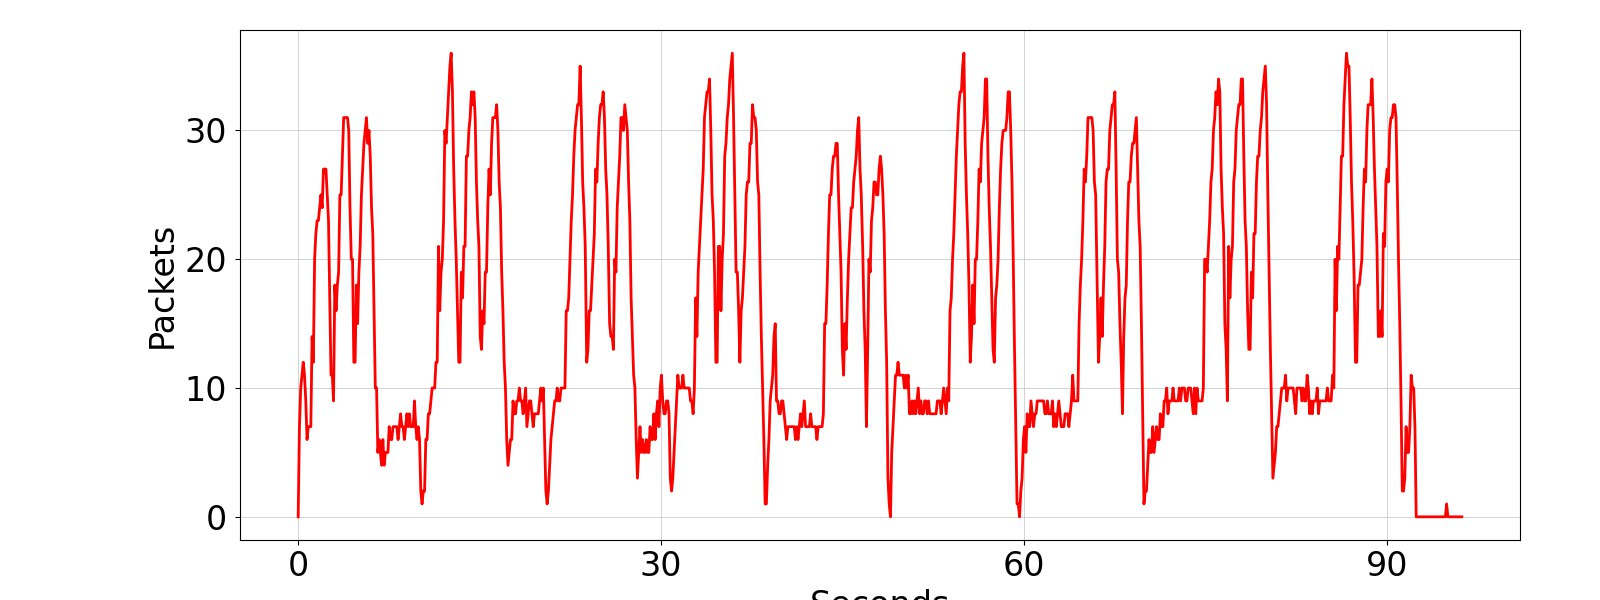
\includegraphics[width=0.7\columnwidth]{./bufferbloat/bb-q100/bbr-buffer.jpg}
  \caption{Número de pacotes na fila do switch ao longo do teste.}
\end{figure}


\subsection{Compare o tempo de busca da página web entre q=20 e q=100 da Parte 3. Qual tamanho da fila fornece um tempo de busca menor? Como isso é diferente da Parte 2?}

Vemos que o tempo quando \code{q=100} é consideravelmente menor do que quando \code{q=20} - aproximadamente 40\% mais rápido. Esse resultado contrasta com o método de controle de congestão Reno, onde a fila maior causa tem um tempo médio 3 vezes maior.

\subsection{Você vê a diferença nos gráficos de tamanho de fila da Parte 2 e da Parte 3? Dê uma breve explicação para o resultado que você vê.}

No gráfico do método Reno, vemos que tanto o RTT quanto o tamanho do buffer tendem a sempre crescer, e nunca voltam a um estado ``vazio''. No caso do BBR, vemos que, ainda que o buffer fique cheio (no caso \code{q=20}) ele ainda sim tende a voltar para um estado vazio, sem crescimento indefinido. Por isso, vemos que o tempo médio de resposta no caso \code{q=100} do BBR não possui quase nenhuma variância, tendo um desvio padrão de apenas 0,05. É importante ressaltar também que o método BBR teve tempo de resposta médio consideravelmente menor, em ambos os casos testados.

\subsection{Você acha que resolvemos o problema do bufferbloat? Explique seu raciocínio.}

O caso de estudo utilizado é simplório demais para que possamos afirmar com certeza que o problema do bufferbloat é resolvido pelo algoritmo BBR, pois só considera um caso específico de fluxo contínuo de pacotes TCP, com latência não muito importante. Para determinar se o bufferbloat fora resolvido, seria necessário analizar uma ampla gama de casos mais complexos, envolvendo sistemas com fluxo sensível à latência e com muito mais pacotes (por exemplo, \textit{streaming} de vídeo ou acesso de muitas pessoas à internet).

Ainda sim, para o caso testado, vemos que o buffer nunca chega a ficar cheio sob o BBR no caso \code{q=100}, com um máximo de 35 a 40 pacotes na fila. Logo, podemos concluir que, para esse caso específico, o método TCP BBR resolve sim o bufferbloat, pois aumentar o buffer não implica em piora da qualidade do sistema - pelo contrário, significou melhora no tempo médio de resposta.

\section{Parte 4}

Para analisar o protocolo QUIC, algumas modificações foram feitas ao arquivo \code{bufferbloat.py}, para utilizar binários gerados pela implementação do protocolo do Cloudflare em Rust, chamada \href{https://github.com/cloudflare/quiche}{quiche}. Assim, o arquivo \code{bufferbloat\_quic.py} apresenta as seguintes modificações:
\begin{enumerate}
\item A implementação do servidor, que antes era feita rodando \code{python webserver.py}, passa a ser feita pelo binário \code{~/redes/bin/quiche-server}. Para gerá-lo, clonamos o repositório do quiche, seguindo as instruções do repositório, e rodamos
\begin{verbatim}
cd <quiche-repositorio>
cargo build --bin quiche-server --target-dir \texttildelow/redes/bin
\end{verbatim}
\item A implementação do cliente, que antes era feita rodando \code{curl}, passa a ser feita pelo binário \code{\texttildelow/redes/bin/quiche-client}. Para gerá-lo, rodamos 
  \begin{verbatim}
cd <quiche-repositorio>
cargo build --bin quiche-client --target-dir \texttildelow/redes/bin
\end{verbatim}
\item A implementação do \code{iperf} fora trocada pelo binário \href{https://github.com/rbruenig/qperf}{qperf}, para medir a performance da rede, já que a ferramenta \code{iperf} não consegue, por padrão, entender o protocolo QUIC.
\end{enumerate}

Ao rodar o arquivo modificado, geramos o seguinte gráfico para o caso \code{q=20}:

\begin{figure}[ht!]
  \centering
  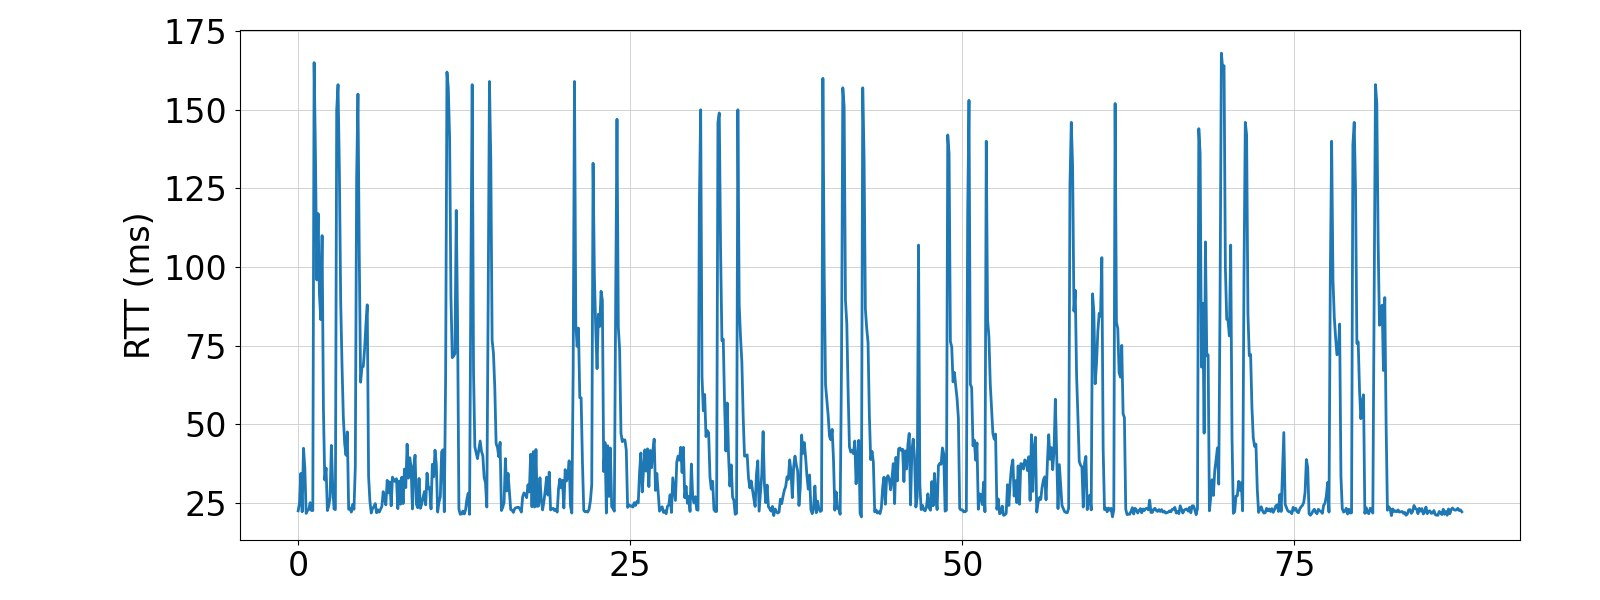
\includegraphics[width=0.5\columnwidth]{./bufferbloat/bb-q20/quic-rtt.jpg}
  \caption{Tempo de resposta dos pings ao longo da duração do teste.}
  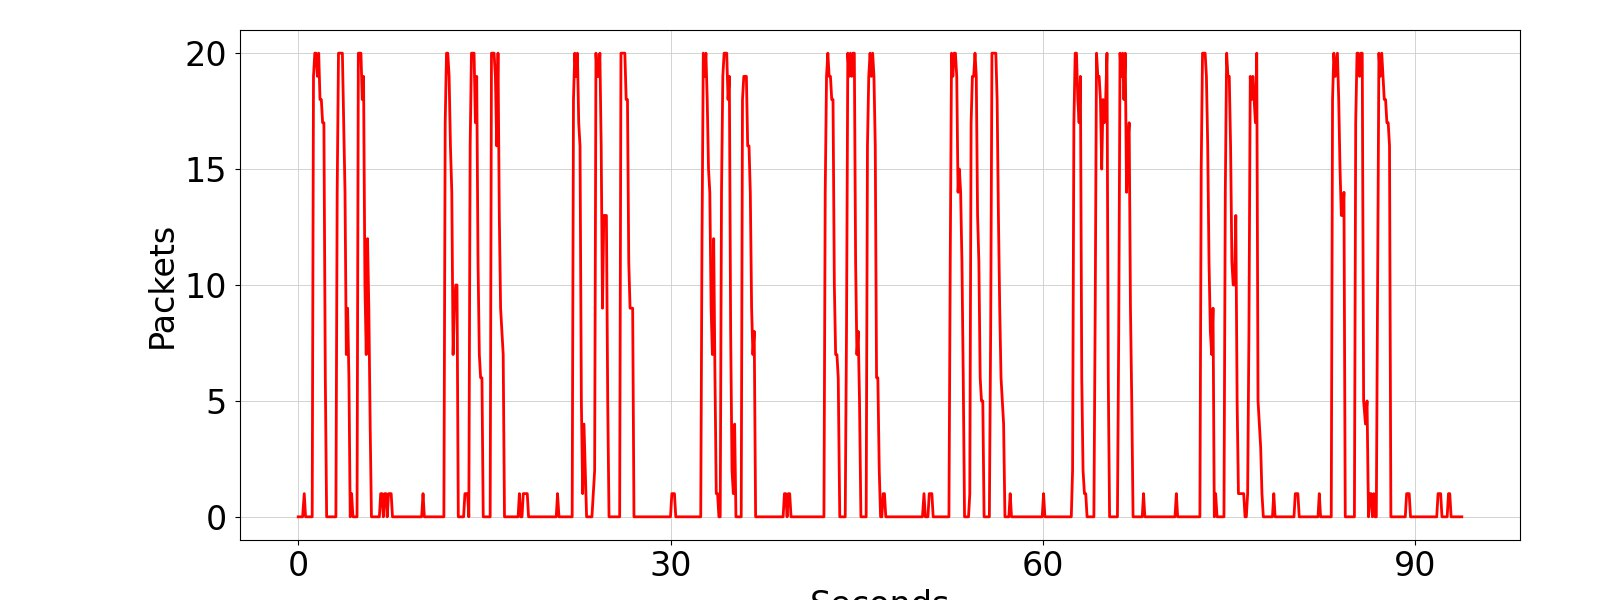
\includegraphics[width=0.5\columnwidth]{./bufferbloat/bb-q20/quic-buffer.jpg}
  \caption{Número de pacotes na fila do switch ao longo do teste.}
\end{figure}

Vemos que o tempo médio de resposta é de 1,76 segundos, com desvio padrão de 0,15. Respectivamente, para o caso \code{q=100}:

\begin{figure}[ht!]
  \centering
  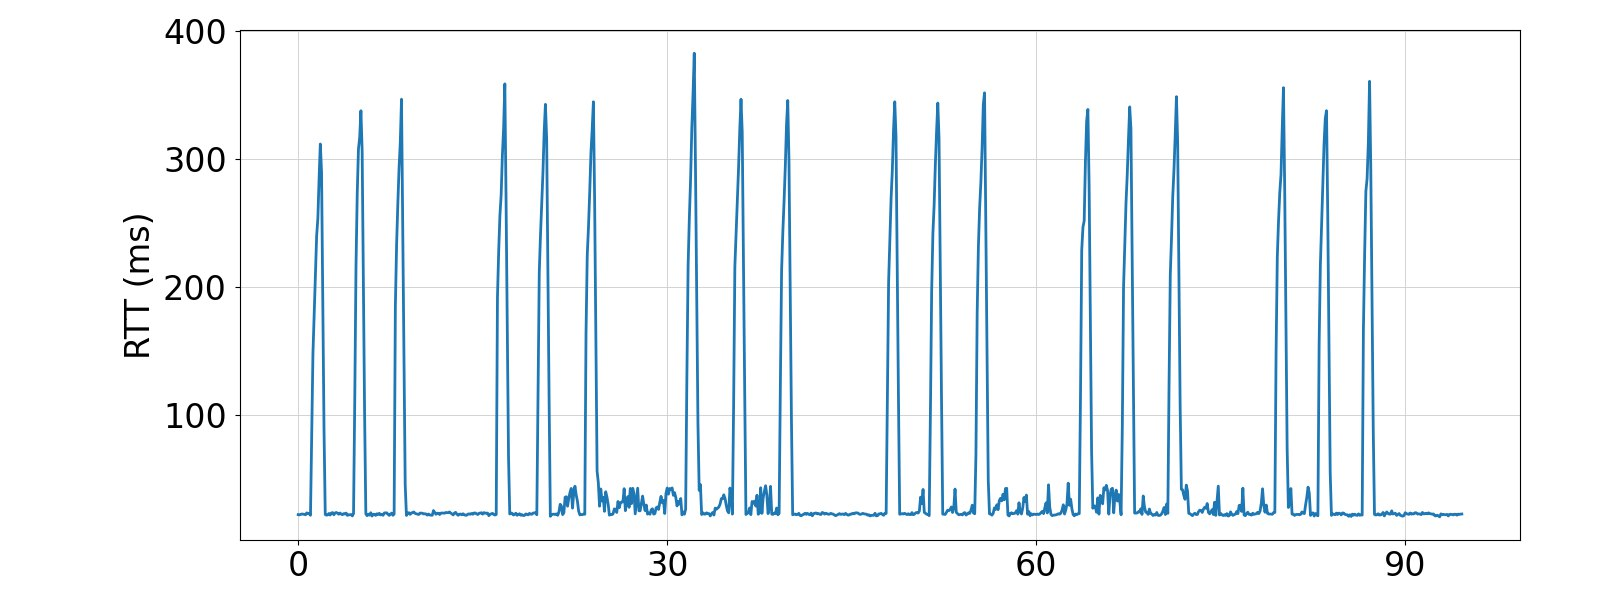
\includegraphics[width=0.5\columnwidth]{./bufferbloat/bb-q100/quic-rtt.jpg}
  \caption{Tempo de resposta dos pings ao longo da duração do teste.}
  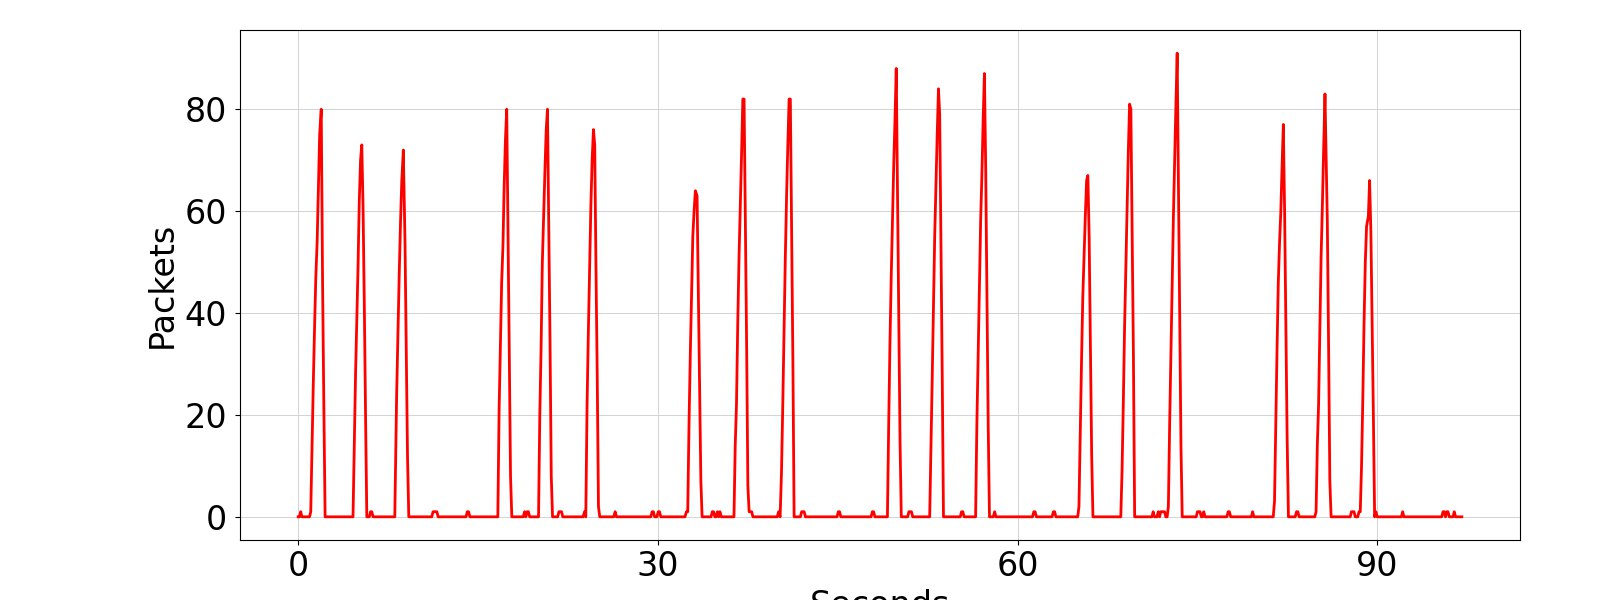
\includegraphics[width=0.5\columnwidth]{./bufferbloat/bb-q100/quic-buffer.jpg}
  \caption{Número de pacotes na fila do switch ao longo do teste.}
\end{figure}

Vemos que o tempo médio de resposta é de 3,66 segundos, com desvio padrão de 0,17.

Notamos que, assim como o TCP Reno, o tamanho do buffer ser maior implicou em um tempo médio de resposta maior, ou seja, o bufferbloat ainda está presente. Apesar disso, vemos que as características dos gráficos são muito distintas, através dos gráficos mais pontiagudos com quedas abruptas do número de pacotes no buffer.

Isso pode ser explicado pela diferença entre o protocolo UDP e TCP. No protocolo TCP, há contínua comunicação entre ambos os lados, tanto do que manda os pacotes segmentados quanto pelo lado que os recebe, respondendo com pacotes de reconhecimento de chegada de cada pacote. Por outro lado, pacotes UDP não possuem nenhum tipo de proteção contra corrupção ou perda de pacotes, e podem ser vistos como pacotes isolados na rede. Como o QUIC utiliza UDP, é esperado que a quantidade de pacotes na rede deva ser consideravelmente menor, e como não há resposta do servidor, quando os pacotes são enviados a fila rapidamente esvazia.

Vemos também que, apesar de sofrer do problema de \textit{bufferbloat}, o protocolo QUIC não só é muito mais rápido mas também muito mais estável do que o protocolo TCP Reno para este caso estudado. Assim, ele deve com certeza ser considerado como um forte candidato para casos onde várias conexões devem ser feitas concorrentemente.



\section{Parte 5}

Para esta seção, escolhemos a opção 1: simulamos a transferência de arquivos pequenos e frequentes. Para isso, colocamos alguns arquivos pequenos (entre 10 e 60KB) na pasta \code{part5} e colocamos 10 hosts na rede requisitando, aleatoriamente, algum desses arquivos ao host h1, com intervalo de um décimo de segundo entre cada requisição. Ao todo, durante o teste, cada um dos 10 hosts clientes requisita 10 arquivos ao host 1.

Para conseguirmos monitorar a fila no switch, fizemos uma mudança na topologia: O host h1 segue conectado ao switch s0, com banda de 1Gb/s. Mas o switch 0 passa a estar conectado ao switch 1, com um link (gargalo) de banda 1.5Mb/s. Esse switch está conectado aos hosts 2, 3, 4... 11 com um link também de 1.5Mb/s. Assim, enquanto os hosts 2 ao 10 fazem as requisições, monitoramos a fila do switch 0 no link entre este switch e o switch 1. Note que o tráfego de todas as requisições ao host 1 passará por lá. 

Fizemos o mesmo teste utilizando QUIC, BBR e Reno. 

\subsection{QUIC}

O código para a parte do QUIC se encontra no arquivo $bufferbloat_quic_part5.py$, que é executado pelo script $run_quic_part5.sh$.

Com a fila máxima em 20 pacotes, houve congestão nesta simulação, como se pode ver na imagem, com a fila atingindo frequentemente os 20 pacotes. Mas a rede se recuperou rapidamente dos eventuais \textit{timeouts}, e a quantidade de pacotes na fila (que reflete as janelas de congestão dos hosts), voltou rapidamente aos 20 pacotes apesar das quedas abruptas. 

Observamos uma média de aproximados 1.81 segundos para recuperar os arquivos, com desvio padrão de 1.96.

\begin{figure}[ht!]
  \centering
  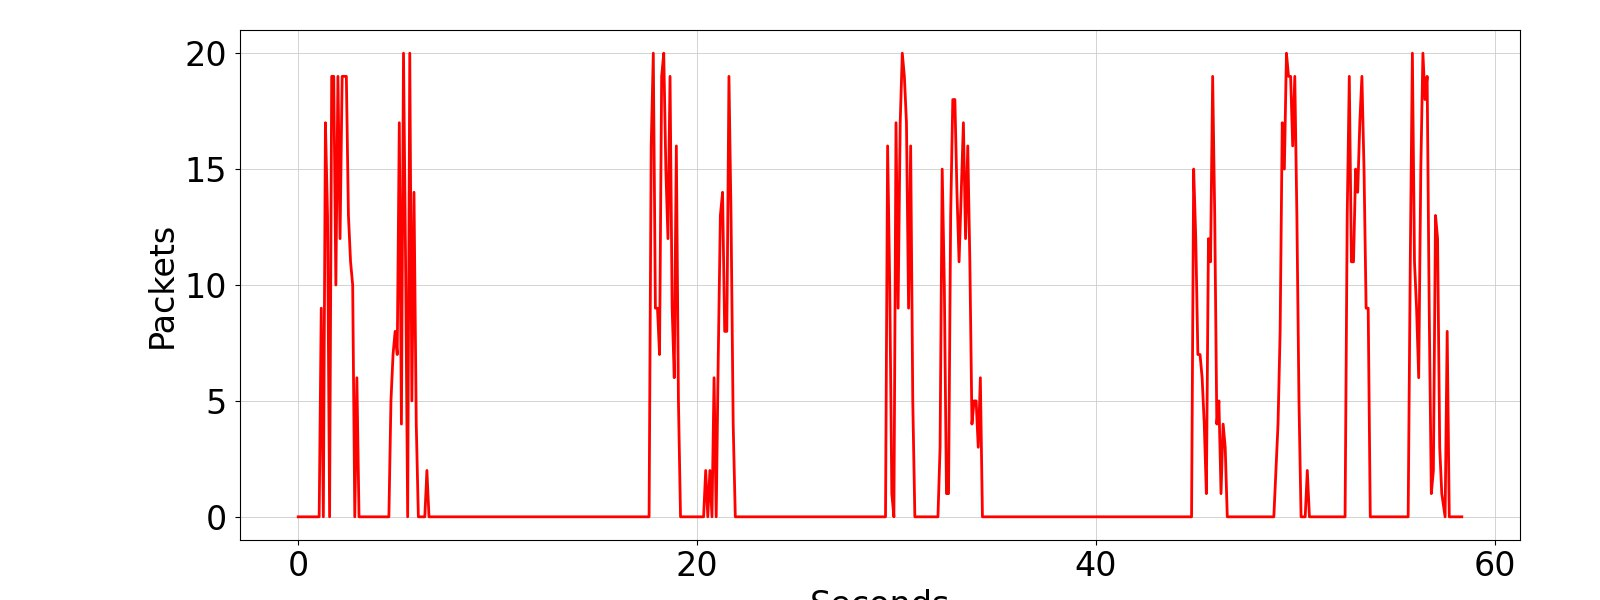
\includegraphics[width=0.5\columnwidth]{./bufferbloat/bb-q20/quic-part5-buffer-q20.jpg}
  \caption{Número de pacotes na fila do link gargalo do switch 0 com tamanho máximo da fila igual a 20 pacotes.}
\end{figure}


Com a fila máxima em 100 pacotes, vimos que a fila não chegou a ficar cheia, e os picos no número de pacotes parecem refletir um fluxo na rede que não chegou a congestionar completamente o switch. Desta forma, nota-se que para efeitos dessa simulação, a rede sob o protocolo QUIC foi capaz de lidar com o fluxo na rede. Mas é interessante observar que, mesmo com a fila maior que não ficou cheia, o tempo médio para recuperar os arquivos não melhorou significativamente (sendo um pouco maior, na verdade), com uma média de 1.84 segundos, e desvio padrão igual a 2.26.

\begin{figure}[ht!]
  \centering
  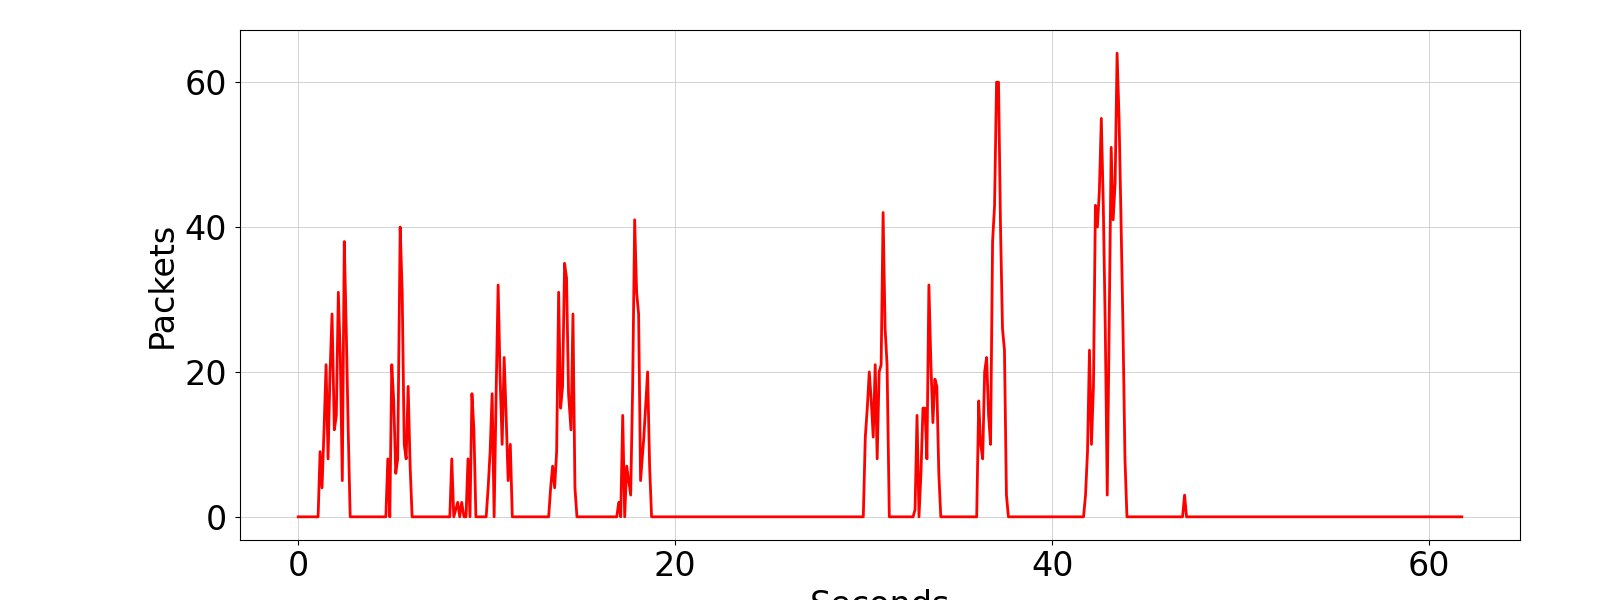
\includegraphics[width=0.5\columnwidth]{./bufferbloat/bb-q100/quic-part5-buffer-q100.jpg}
  \caption{Número de pacotes na fila do link gargalo do switch 0 com tamanho máximo da fila igual a 100 pacotes.}
\end{figure}

\subsection{BBR}

O código para a parte do BBR se encontra no arquivo $bufferbloat_bbr_part5.py$, que é executado pelo script $run_bbr_part5.sh$.

Como no exemplo do QUIC, fica claro que no BBR tambem tivemos uma amostra de congestionamento em alguns momentos indicado pela variação na taxa de transmissao e pela latencia. Vemos tambem como BBR  mais agressivo, no tratamento dos congestionamentos, percebemos pelos picos acentuados . 

Observamos uma média de aproximados 0.5 segundos para recuperar os arquivos, com desvio padrão de 0.39.


\begin{figure}[ht!]
	\centering
	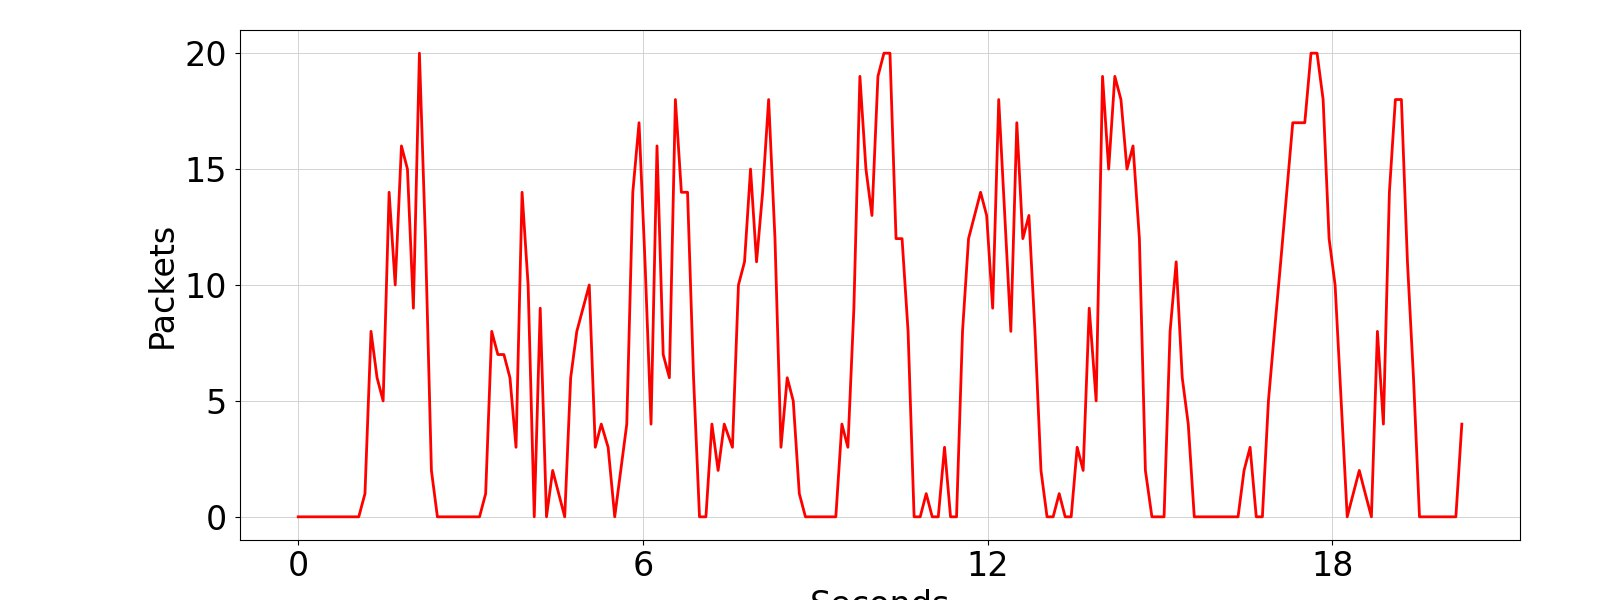
\includegraphics[width=0.5\columnwidth]{./bufferbloat/bb-q20/bbr-part5-buffer-q20.jpg}
	\caption{Número de pacotes na fila do link gargalo do switch 0 com tamanho máximo da fila igual a 20 pacotes.}
\end{figure}

Importante salientar que por conta da natureza do fluxo o buffer nunca de fato chegou a 100


Com uma média de 1.84 segundos, e desvio padrão igual a 0.22.

\begin{figure}[ht!]
	
	\centering
	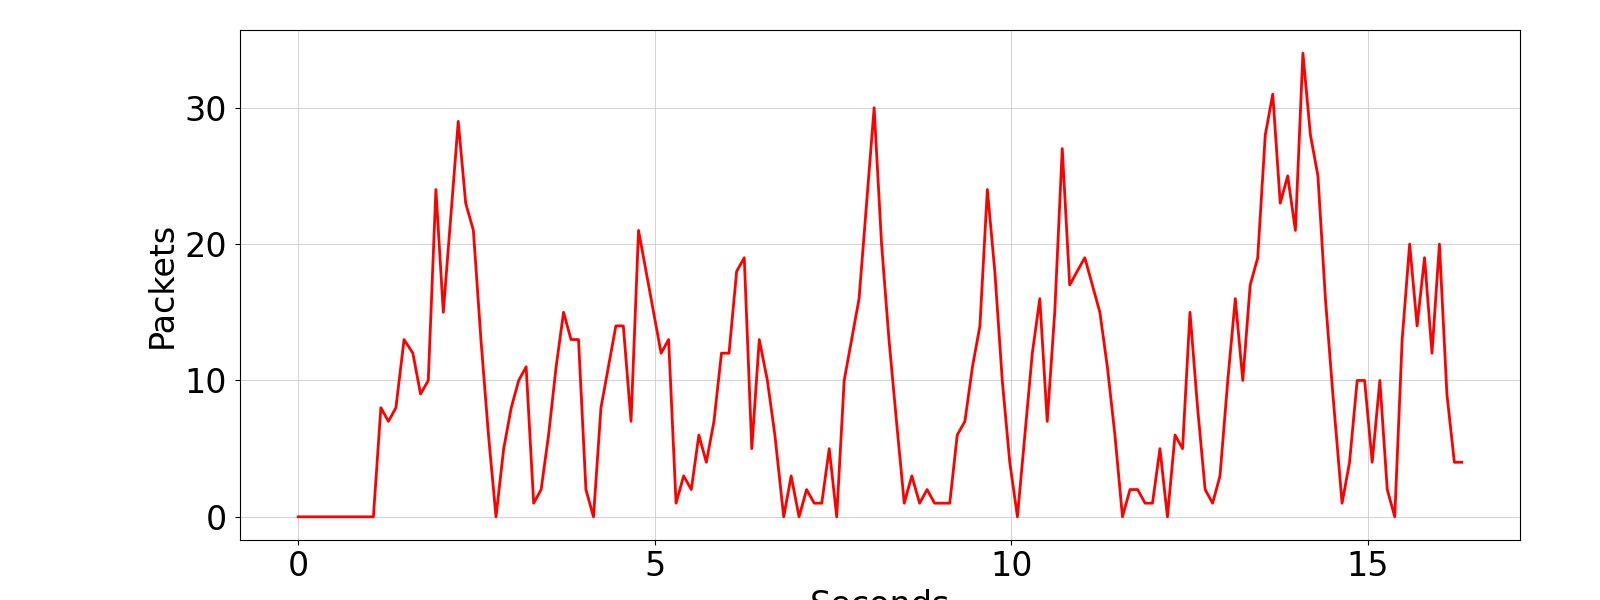
\includegraphics[width=0.5\columnwidth]{./bufferbloat/bb-q100/bbr-part5-buffer-q100.jpg}
	\caption{Número de pacotes na fila do link gargalo do switch 0 com tamanho máximo da fila igual a 100 pacotes.}
\end{figure}

\subsection{RENO}

O código para a parte do RENO se encontra no arquivo $bufferbloat_reno_part5.py$, que é executado pelo script $run_reno_part5.sh$.

Vemos como o RENO se difere do BBR com picos mais constantes e vales tambem mais prolongados, pois sua natureza e menos agressiva ao tratar os congestionamentos 

Observamos uma média de aproximados 0.45 segundos para recuperar os arquivos, com desvio padrão de 0.33.

\begin{figure}[ht!]
	\centering
	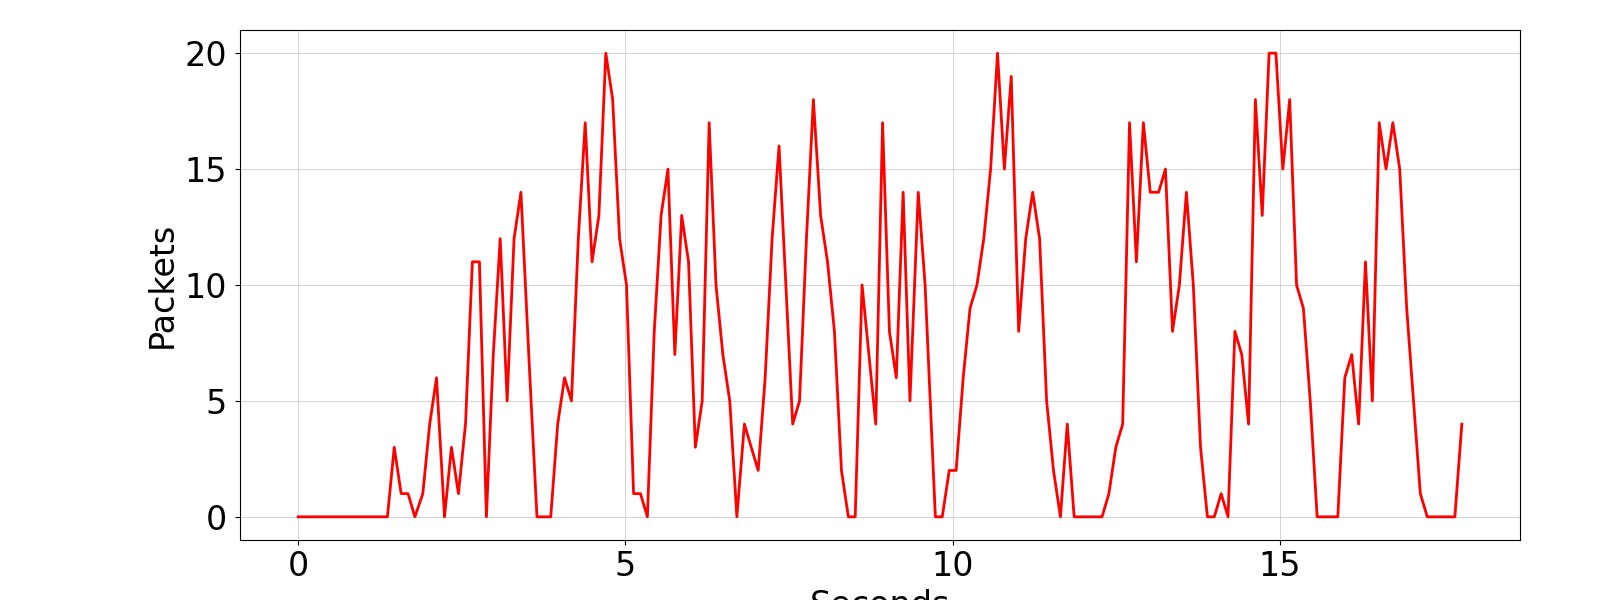
\includegraphics[width=0.5\columnwidth]{./bufferbloat/bb-q20/reno-part5-buffer-q20.jpg}
	\caption{Número de pacotes na fila do link gargalo do switch 0 com tamanho máximo da fila igual a 20 pacotes.}
\end{figure}


Com uma média de 0.58 segundos, e desvio padrão igual a 0.33.

\begin{figure}[ht!]
	\centering
	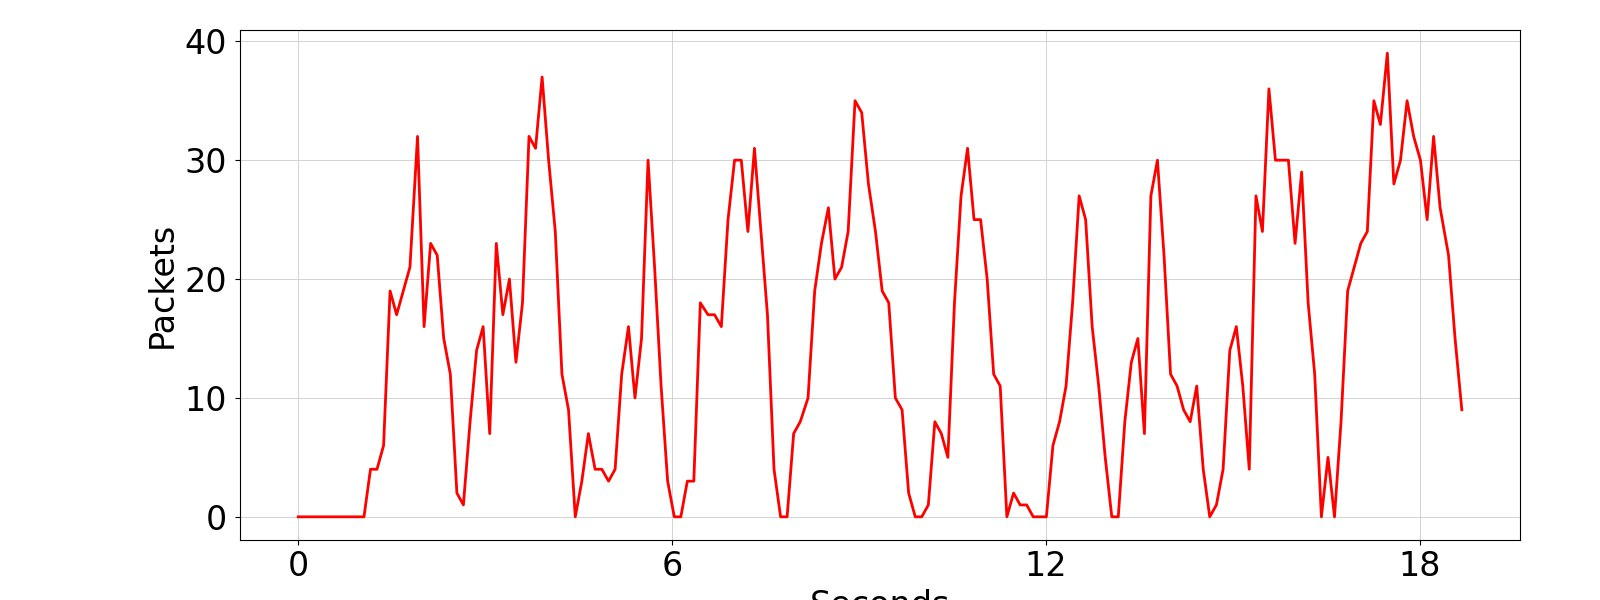
\includegraphics[width=0.5\columnwidth]{./bufferbloat/bb-q100/reno-part5-buffer-q100.jpg}
	\caption{Número de pacotes na fila do link gargalo do switch 0 com tamanho máximo da fila igual a 100 pacotes.}
\end{figure}




\subsection{Respostas}

1. Essa resposta pode depender do fluxo na rede, e também do mecanismo de controle de congestão utilizado. Claro, se conhecermos o número de fluxos passando pelo roteador, podemos fazer como mencionado no item 5 e definir o tamanho do buffer como RTT * C/sqrt(N), ou fazer uma estimativa para N. é importante lembrar que buffers muito grandes podem levar justamente ao problema do bufferbloat, com esperas muito longas em fila, além de timeouts desnecessários gerando menor "goodput"

2. Porque o tamanho ótimo do buffer de um roteador pode mudar a depender do fluxo na rede, fluxo este que será influenciado por elementos da camada de rede como os mecanismos de roteamento; e diferentes protocolos da camada de transporte, por exemplo os diferentes algoritmos de controle de congestão do TCP, vão influenciar como o buffer será utilizado. No BBR, por exemplo, a tendência é reduzir a transmissão de dados antes do buffer ficar  muito cheio. As diferentes formas de se recuperar de perdas também impactam os buffers,  como AIMD vs cubic.

3. Não. Em si, aumentar o tamanho do buffer não leva necessariamente ao aumento de throughput. Este depende da capacidade de transmissão nos links envolvidos. O que pode ocorrer com o  aumento de buffer (e consequente ocorrência de bufferbloat) é a diminuição do goodput, uma vez que pelo aumento do tempo de espera em fila, pode haver timeouts que não refletem uma perda, gerando mais pacotes sendo enviados que reflitam um mesmo dado. De fato há uma tendência de haver menos perdas por falta de espaço em buffer. Mas o bufferbloat pode gerar aumento do delay (em específico, o delay entre enviar um dado pela rede e este ser corretamente recebido).

4. Sim. Isso é descrito no item anterior, por estar relacionado com redução do goodput.	

5. Essa proposta, que era inicialmente RTT*C, tinha o intuito de estimar que, com uma capacidade do link de C bits/s e um round-trip-time de RTT segundos, seriam enviados C bits por segundo a cada RTT segundos, resultando na necessidade de se acomodar C bits no buffer do roteador. Como  pode haver N fluxos diferentes na rede, surgiu a proposta mais "completa" de RTT*C/sqrt(N).  Um controlador SDN pode ser útil para observar os fluxos na rede e estimar, através dos cabeçalhos (com diferentes endereços), a quantidade de fluxos na rede a cada intervalo de tempo para atualizar o espaço em buffer.

6. O tamanho do buffer pode mudar ao longo do tempo no sentido de que o roteador pode ter um certo tamanho máximo, físico, do seu buffer, é físico, mas o roteador pode ter limites diferentes ao longo do tempo para  o espaço alocado para a fila, de modo a empregar estratégias que usam o tamanho do buffer para reduzir a latência na rede. 

\end{document}
